\documentclass[conference]{IEEEtran}
\IEEEoverridecommandlockouts

% Core Packages
\usepackage{cite}
\usepackage{amsmath,amssymb,amsfonts}
\usepackage{algorithmic}
\usepackage{graphicx}
\usepackage{textcomp}
\usepackage{xcolor}
\usepackage{array}
\usepackage{booktabs}
\usepackage{url}
\usepackage{stmaryrd}
\usepackage{comment}
\usepackage{float}
\usepackage{placeins}
\usepackage{tikz}
\usetikzlibrary{arrows.meta}
\usepackage{pgfplots}
\usepgfplotslibrary{groupplots}
\usetikzlibrary{calc}
\pgfplotsset{compat=1.18}

% Custom Macros & Placeholders
\def\BibTeX{{\rm B\kern-.05em{\sc i\kern-.025em b}\kern-.08em
    T\kern-.1667em\lower.7ex\hbox{E}\kern-.125emX}}

\newcommand{\phfig}[2]{\fbox{\parbox[c][#1][c]{0.92\columnwidth}{\centering\small #2}}}
\newcommand{\phfigwide}[2]{\fbox{\parbox[c][#1][c]{0.96\textwidth}{\centering\small #2}}}
\newcommand{\figph}[2]{\fbox{\parbox[c][#1][c]{0.92\columnwidth}{\centering\small #2}}}
\newcommand{\figphwide}[2]{\fbox{\parbox[c][#1][c]{0.96\textwidth}{\centering\small #2}}}

\begin{document}

% ---- Float placement tuning (prevents figures from landing on blank pages) ----
\renewcommand{\topfraction}{0.9}      % max fraction of page for top floats
\renewcommand{\bottomfraction}{0.8}   % max fraction of page for bottom floats
\renewcommand{\textfraction}{0.07}    % min fraction of page that must be text
\renewcommand{\floatpagefraction}{0.7}% min fraction filled on a float-only page
\setcounter{topnumber}{4}
\setcounter{bottomnumber}{4}
\setcounter{totalnumber}{6}
% -------------------------------------------------------------------------------

\title{Model Compression and Input Optimization Co-Design for Edge Driver Monitoring Systems}

\author{
  \IEEEauthorblockN{1\textsuperscript{st} Oumar Mamoun Ibrahim}
  \IEEEauthorblockA{\textit{Department of Computer Engineering} \\
  \textit{University of Sharjah} \\
  Sharjah, UAE \\
  U22200741@sharjah.ac.ae}
  \and
  \IEEEauthorblockN{2\textsuperscript{nd} Mohamad Khairi bin Ishak}
  \IEEEauthorblockA{\textit{Department of Computer Engineering} \\
  \textit{University of Sharjah} \\
  Sharjah, UAE \\
  mishak@sharjah.ac.ae}
  \and
  \IEEEauthorblockN{3\textsuperscript{rd} Ahmed Atef Abouelhamd}
  \IEEEauthorblockA{\textit{Department of Computer Engineering} \\
 \textit{University of Sharjah} \\
 Sharjah, UAE \\
 U23104122@sharjah.ac.ae}
}

\maketitle

\begin{abstract}
Edge-deployed driver monitoring systems (DMS) must detect distraction and drowsiness cues in real time under strict latency, memory, and power budgets, yet most object detectors are designed for high-performance hardware. We study this gap through a three-phase evaluation of nano-scale YOLO detectors on the Driver Monitoring Dataset (DMD), using a subject-disjoint 8:3:3 split, four driver-behavior classes, and macro-recall as the primary safety metric. Phase~I evaluates structured $\ell_1$-norm channel pruning (10--90\% sparsity) combined with INT8 post-training quantization (PTQ) and quantization-aware training (QAT). YOLO11n remains within the 5-pp safety recall floor up to 70\% pruning (85.6\% vs.\ 86.4\% baseline), whereas YOLO26n holds only up to 60\%; in single-seed runs, PTQ INT8 preserves recall at 70\% sparsity. Phase~II compares a static central $400\times400$ crop with a $640\times640$ overlapping collage across input resolutions from $640\times640$ down to $80\times80$. The $320\times320$ crop gives the best trade-off, matching the full-frame macro-F1 at one quarter of the GFLOPs. Phase~III co-designs a 70\%-pruned, PTQ INT8 YOLO11n on a $320\times320$ cropped input requires 0.614~GFLOPs and 1.19~MB, a $10.6\times$ compute and $4.4\times$ storage reduction, at 92\% of the baseline macro-recall. Our results show that DMS object detection can be made more compute efficient through model-side and input-side optimization at a marginal recall loss.
\end{abstract}

\begin{IEEEkeywords}
Object Detection, Driver Monitoring Systems, Edge Deployment, Model Pruning, Quantization, Region-of-Interest
\end{IEEEkeywords}


\section{Introduction}
Most computer vision models are designed for high-performance systems, which increases neural network size and the computation and storage required for inference~\cite{b1}, making direct deployment on edge devices impractical~\cite{b2,b3}. To bridge this gap, practitioners apply targeted optimizations that adapt models to constrained hardware, principally model pruning~\cite{b4}, quantization~\cite{b5}, and knowledge distillation~\cite{b6}. These methods reduce the parameter count and inference cost from different angles. Edge-deployed driver monitoring systems are particularly demanding: the object detection model must evaluate every frame in real time to catch distraction and drowsiness cues without latency spikes.

In this work, we address a central research question:
\begin{itemize}
    \item How do model-level compression and input-level preprocessing compare in isolation, and can their co-design outperform standard baselines in edge efficiency without violating safety-critical recall?
\end{itemize}

We approach the question from two orthogonal sides involving the model and the input. Later to combine both into a proposed co-designed pipeline, evaluated against their official baselines.

On the model side, we evaluate structured $\ell_1$-norm magnitude pruning, which ranks convolutional channels by their weight magnitudes and removes the least significant ones~\cite{b9}. Structured pruning directly reduces floating-point operations (FLOPs) and inference latency on commodity hardware, and is compatible with quantization without requiring specialized sparse accelerators. We also evaluate post-training quantization (PTQ) and quantization-aware training (QAT), which convert network weights from 32-bit floating-point to INT8, cutting memory traffic and checkpoint size.

On the input side, we explore two preprocessing strategies applied to the native $640\times640$ Driver Monitoring Dataset (DMD) frames:
\begin{itemize}
    \item A static central $400\times400$ Region-of-Interest (RoI) crop, subsequently scaled to the target network resolution.
    \item A static overlapping frame collage at the native $640\times640$ resolution with 25\% pixel overlap.
\end{itemize}
Both strategies are evaluated across a geometric resolution sweep ($640$, $320$, $160$, $80$ pixels) using bilinear interpolation.

The main contributions of this paper are:
\begin{itemize}
    \item An ablation study of $\ell_1$-norm structured pruning and INT8 quantization (PTQ and QAT) on YOLO11n and YOLO26n, reporting macro-recall, per-class recall, GFLOPs, and checkpoint size as a function of sparsity.
    \item An ablation study of two static RoI input preprocessing strategies across four network input resolutions, with accuracy and latency measured end-to-end on an NVIDIA RTX~4060.
    \item A comprehensive benchmark of the proposed co-designed system involving a 70\% pruned YOLO11n with PTQ INT8 at a $320\times320$ cropped input (0.614~GFLOPs, 1.19~MB) and at a $160\times160$ cropped input (0.153~GFLOPs, 1.16~MB) against native FP32 YOLO baselines.
\end{itemize}


\section{Related Work}

\subsection{Model Compression for Edge Object Detection}
Deploying detectors on embedded hardware relies on three main techniques: pruning, quantization, and efficient architecture design. Unstructured pruning removes individual low-magnitude weights~\cite{b8}, but the resulting sparsity seldom yields real speedups on commodity accelerators. Structured pruning removes entire filters or channels, producing a smaller dense network that runs faster without sparse hardware support. Li \emph{et al.}\ \cite{b9} rank filters by their $\ell_1$ norm and discard the weakest; He \emph{et al.}\ \cite{b10} select channels through LASSO regression with feature-map reconstruction; and Liu \emph{et al.}\ \cite{b11} exploit sparsity in batch-normalization scale factors. Fang \emph{et al.}\ \cite{b12} extend structural pruning to arbitrary architectures through dependency graphs which is an important property for modern YOLO models whose concatenations and residual links couple channels across layers.

Quantization lowers numerical precision to cut memory traffic and latency. Jacob \emph{et al.}\ \cite{b13} introduced integer-arithmetic-only inference with QAT, and Krishnamoorthi~\cite{b14} compared PTQ and QAT for INT8 deployment. Han \emph{et al.}\ \cite{b8} showed that pruning and quantization are complementary when applied jointly.

The YOLO family is a standard choice for real-time detection on constrained devices. YOLOv7 introduced trainable bag-of-freebies and planned re-parameterization~\cite{b15}. YOLOv10 removed non-maximum suppression through consistent dual assignments and a holistic efficiency-driven design~\cite{b16}. YOLO11 introduced C3k2 and C2PSA blocks~\cite{b17}. Compression studies of these detectors typically report mean average precision on general-purpose benchmarks; recall on safety-critical minority classes receives far less attention.

\subsection{Input-Level and RoI Optimization}
Input resolution is a primary driver of inference cost, so cropping, tiling, and resolution selection are natural levers for real-time systems. Unel \emph{et al.}\ \cite{b18} showed that tiling improves small-object detection. Najibi \emph{et al.}\ \cite{b19} proposed AutoFocus, which processes only selected high-resolution regions to save computation. These methods target generic scenes in which object locations are unpredictable. In an in-cabin camera, the driver's upper body occupies a predictable region of the frame, making static RoI selection like a central crop or an overlapping collage a natural design choice. To our knowledge, such strategies have not been compared systematically across input resolutions for in-cabin behavior detection.

\subsection{Driver Monitoring Systems}
Deep learning has become the standard approach to driver distraction and drowsiness detection. The Driver Monitoring Dataset (DMD)~\cite{b20} provides multi-modal in-cabin recordings with annotated attention and alertness states, and serves as a common benchmark. Abouelnaga \emph{et al.}\ \cite{b21} studied real-time distracted driver posture classification and treated inference speed as a design constraint. Kashevnik \emph{et al.}\ \cite{b22} surveyed driver distraction detection methods and organized them into a common framework. 
\subsection{Research Gap}
Existing work treats compression, input-level optimization, and driver monitoring largely in isolation. To the best of our knowledge, no prior work has jointly evaluated structured pruning and quantization together with input-level RoI strategies for edge-constrained DMS. This paper addresses that gap. It benchmarks structured $\ell_1$ channel pruning and INT8 quantization (PTQ and QAT) on two sub-3M-parameter YOLO models; evaluates central-crop and overlapping-collage inputs across four resolutions; and co-designs the best compressed model with the best input strategy, with recall as the primary safety metric.

The main gaps are summarized below (see also Table~\ref{tab:gap}):
\begin{itemize}
    \item Compression studies of YOLO-family detectors typically target mean average precision on general-purpose benchmarks, and recall on safety-critical minority classes receives far less attention.
    \item Static RoI strategies such as a central crop or an overlapping collage have not been compared systematically across input resolutions for in-cabin behavior detection.
    \item No prior work has evaluated the combined effect of pruning, quantization, and input-level RoI preprocessing on edge-constrained deployment of DMS.
\end{itemize}
\begin{table}[t]
\caption{Coverage of prior work versus this paper. A checkmark indicates the aspect is addressed; ``Joint'' denotes combined evaluation of all preceding aspects.}
\label{tab:gap}
\centering
\footnotesize
\setlength{\tabcolsep}{3pt}
\begin{tabular}{@{}lccccc@{}}
\toprule
\textbf{Work} & \textbf{Pruning} & \textbf{Quant.} & \textbf{RoI} & \textbf{DMS} & \textbf{Joint} \\
\midrule
Filter/channel pruning \cite{b9,b10,b11,b12} & $\checkmark$ & -- & -- & -- & -- \\
Deep compression \cite{b8}                   & $\checkmark$ & $\checkmark$ & -- & -- & -- \\
Quantization \cite{b13,b14}                  & -- & $\checkmark$ & -- & -- & -- \\
Tiling / multi-scale RoI \cite{b18,b19}      & -- & -- & $\checkmark$ & -- & -- \\
DMS / distraction \cite{b20,b21,b22}         & -- & -- & -- & $\checkmark$ & -- \\
\midrule
\textbf{This work} & $\checkmark$ & $\checkmark$ & $\checkmark$ & $\checkmark$ & $\checkmark$ \\
\bottomrule
\end{tabular}
\end{table}


\section{Methodology}

To isolate the effect of each optimization, the main experiment is divided into three phases. Phase~I explores an ablation study on the effects of structured pruning and INT8 quantization on primary detection metrics. Phase~II explores an ablation study on two input preprocessing methods across a resolution sweep. Phase~III concludes with a joint co-design proposed in this paper, evaluated against native baselines.

\subsection{Models and Dataset}
The primary lightweight model evaluated is YOLO11n, a compact architecture integrating C3k2 blocks and C2PSA spatial attention with 2.59M parameters and 6.50~GFLOPs at $640\times640$ input. In Phase~I, we additionally evaluate YOLO26n, a latency-optimized detector using re-parameterized convolutions and an efficient neck topology, with 2.51M parameters and 5.90~GFLOPs. The primary dataset is the Driver Monitoring Dataset (DMD), which contains in-cabin $1280\times720$ RGB video footage from 14 subjects performing drowsy and distracted driving. A total of 15{,}723 frames are extracted at 1~FPS from the videos and center-cropped to the baseline $640\times640$ resolution. The dataset is split at the subject level with a ratio of 8:3:3 for training (subjects~01, 04, 06--09, 13, 14; 9{,}087 frames), validation (subjects~02, 03, 11; 3{,}423 frames), and testing (subjects~05, 10, 12; 3{,}213 frames), with strictly zero subject overlap across splits. Frames are manually annotated by two primary annotators. Negative frames contain no bounding boxes; positive frames contain exactly one localized bounding box identifying one of four driver cues: yawning, hand-over-mouth, drinking, or phone use. Negative frames make up $\approx81\%$ of all frames (12{,}722 frames), and phone-use frames make up $\approx81\%$ of positive frames (2{,}437 frames), creating a severe class imbalance for the three remaining classes. Notably, the held-out test split contains only 33 yawning frames and 28 hand-over-mouth frames, so each missed detection shifts the class recall by 3.0--3.6 percentage points. Unless stated otherwise, all configurations are trained on the eight training subjects and evaluated on the three held-out test subjects across three random seeds to capture training variance, with results reported as mean $\pm$ standard deviation. We define Macro-recall as the unweighted mean of per-class recall and it is treated as the primary safety metric. Mean average precision (mAP) is reported at IoU thresholds of 0.5 (mAP@0.5) and averaged from 0.5 to 0.95 (mAP@0.5:0.95). All models are initialized from COCO pretrained checkpoints and fine-tuned using the Ultralytics framework on an NVIDIA RTX~4060 8\,GB GPU with SGD optimization (batch size 16, initial learning rate $\text{lr}_0 = 0.01$, momentum 0.937, weight decay 0.0005).

\subsection{Model-Side Optimization}
Models are trained from the unpruned (0\%) baseline up to 90\% nominal pruning in 10\% steps. In automotive safety guidelines for DMS \cite{euroncap2026driver,isots5283}, a missed detection of driver distraction or drowsiness is a safety hazard. Conversely, a false detection is merely an annoyance. Recall is therefore prioritized, and a Safety Recall Floor is enforced:
\[
R_{\text{Floor}} = R_{\text{base}} - \delta\quad(\delta=0.05).
\]
Any compressed model dropping more than 5 percentage points of macro-recall from the uncompressed baseline is deemed unsafe. In Phases~I and~III, recall is computed at a fixed confidence threshold of $\tau=0.5$ to suppress sparse, low-confidence detections. Pruning is structured and uses $\ell_1$-norm magnitude ranking to remove low-significance channels. We subsequently train new models using PTQ and QAT. Pruning efficiency is defined as
\[
\text{Eff}_{\text{FLOPs}} = \frac{\text{macro-recall}\,(\%)}{\text{GFLOPs}},
\]
and quantization efficiency as
\[
\text{Eff}_{\text{MB}} = \frac{\text{macro-recall}\,(\%)}{\text{Size (MB)}}.
\]
The Ultralytics \texttt{DetectionTrainer} fine-tunes the pruned architecture. Channels are ranked by the $\ell_1$ norm of their \texttt{Conv2d} filters; the lowest-ranked fraction is removed. Detection heads, spatial attention modules, and layers with fewer than 8 output channels are excluded from pruning. Weights are transferred from C3k2 to C3k2-v2 with exact numerical equivalence.

\subsection{Input-Side Optimization}
\label{sec:threshold}
Orthogonally, the baseline models are evaluated across a geometric progression of input resolutions ($80\times80$, $160\times160$, $320\times320$, $640\times640$, and $1280\times1280$), resampled from the native $640\times640$ frames via bilinear interpolation. Two methods are explored: a static central $400\times400$ RoI cropped from the native frame (coordinates $X\in[140,540]$, $Y\in[120,520]$) and scaled to the target resolution, and a static frame collage with 25\% pixel overlap at the native $640\times640$ resolution. The central crop method reduces the unique pixel count by $\approx61\%$ relative to the baseline frame. The collage method arranges the original frame into three tiles where two square tiles cover the sides of the driver and one elongated tile covers the driver's head, removing the corner pixels of the baseline frame. YOLO requires input side lengths divisible by the maximum stride of 32 so the network therefore pads an $80\times80$ input to $96\times96$. We define F1 as the harmonic mean of precision and recall:
\[
F1_c = \frac{2\,P_c\,R_c}{P_c + R_c},
\]
where $P_c$ and $R_c$ are the precision and recall of class $c$. We average F1 over the four classes to obtain macro-F1:
\[
\text{macro-}F1 = \frac{1}{4} \sum_{c=1}^{4} F1_c.
\]
In Phase~II, for each run we scan the confidence threshold on the validation subjects and pick the value $\tau^*$ that maximizes macro-F1; we then freeze $\tau^*$ and apply it once to the test subjects, so test data never influence threshold selection. % Preprocessing time covers cropping, stitching, and bilinear resizing (for the crop method only), all performed on the CPU. Latency is reported as the additional time a method adds relative to unmodified inference:
%\[
%\Delta t_m = t_m - t_0, \qquad m \in \{\text{collage},\ \text{crop-%expand}\},
%\]
%where $t_m$ is the end-to-end inference time with preprocessing method $m$ and $t_0$ is the time on the original unmodified image. 
Figure~\ref{fig:preprocessing_comparison} shows an example of what each RoI method produces.

\begin{figure}[!t]
    \centering
    \includegraphics[width=\linewidth]{Figure1and2.png}
    \caption{Qualitative comparison of native input frames alongside the resulting outputs of each preprocessing method.}
    \label{fig:preprocessing_comparison}
\end{figure}

\subsection{Joint Co-design}
Phase~III combines the three optimizations studied in Phases~I and~II into a single pipeline: central RoI cropping, 70\% structured pruning, and INT8 PTQ. From the earlier phases, we select the primary deployment candidates: pruned YOLO11n models with PTQ INT8 at $320\times320$ and $160\times160$ cropped inputs (Table~\ref{tab:codesign_study}). These are evaluated against native FP32 baselines at $640\times640$ (YOLO11n and YOLO26n). Unlike Phase~II, no threshold tuning is performed: every model is evaluated at a fixed confidence threshold of $\tau=0.5$, consistent with Phase~I. We report precision and macro-recall as detection metrics, and parameter count, GFLOPs, and model size in MB as cost metrics. % The Safety Recall Floor is applied relative to the native YOLO11n baseline.


\section{Results and Discussion}
\label{sec:results}

\subsection{Phase 1: Model-Side Optimization}

% ======================================================================
% Tab. Main Pruning 
% ======================================================================

\begin{table*}[!t]
\renewcommand{\arraystretch}{0.85}
\caption{Structured $\ell_1$-norm channel pruning test results across 3 seeds at the fixed threshold $\tau = 0.5$. Arrows indicate the better direction; bold marks the best value within each model.}
\label{tab:pruning_fixed_tau}
\centering
\scriptsize
\setlength{\tabcolsep}{2.6pt}
\begin{tabular}{l rrr c cccc c c c}
\toprule
 & \multicolumn{3}{c}{Cost $\downarrow$} & & \multicolumn{4}{c}{Per-class recall (\%) $\uparrow$} & & & \\
\cmidrule(lr){2-4}\cmidrule(lr){6-9}
Sparsity & Params (M) & GFLOPs & Size (MB) & Prec. (\%) $\uparrow$ & Yawning & Hand--mouth & Drinking & Phone use & Macro-recall (\%) $\uparrow$ & $\text{Eff}_{\text{FLOPs}}$ $\uparrow$ & Safe? \\
\midrule
\multicolumn{12}{l}{\textit{YOLO11n}} \\
Base  & 2.59 & 6.50 & 5.23 & $93.6\pm1.2$ & $80.8\pm1.7$ & $92.9\pm3.6$ & $89.3\pm1.8$ & $82.6\pm1.5$ & $86.4\pm1.3$ & 13.3 & YES \\
10\%  & 2.24 & 5.63 & 4.59 & $93.9\pm0.4$ & $80.8\pm6.3$ & $90.5\pm4.1$ & $\mathbf{94.0}\pm\mathbf{4.1}$ & $79.9\pm3.4$ & $86.3\pm3.7$ & 15.3 & YES \\
20\%  & 1.94 & 4.92 & 4.02 & $93.7\pm1.0$ & $83.8\pm7.6$ & $\mathbf{95.2}\pm\mathbf{2.1}$ & $90.5\pm4.1$ & $82.4\pm1.4$ & $88.0\pm2.9$ & 17.9 & YES \\
30\%  & 1.67 & 4.30 & 3.50 & $\mathbf{94.2}\pm\mathbf{0.5}$ & $84.8\pm8.0$ & $92.9\pm0.0$ & $90.5\pm2.7$ & $80.7\pm2.7$ & $87.2\pm2.1$ & 20.3 & YES \\
40\%  & 1.43 & 3.74 & 3.04 & $93.9\pm1.4$ & $76.8\pm6.3$ & $90.5\pm5.5$ & $89.3\pm3.1$ & $81.2\pm1.2$ & $84.4\pm2.3$ & 22.6 & YES \\
50\%  & 1.23 & 3.30 & 2.65 & $93.0\pm1.5$ & $78.8\pm5.2$ & $92.9\pm3.6$ & $89.3\pm0.0$ & $81.5\pm0.9$ & $85.6\pm2.3$ & 25.9 & YES \\
60\%  & 1.04 & 2.84 & 2.29 & $93.1\pm0.5$ & $\mathbf{85.9}\pm\mathbf{7.0}$ & $92.9\pm6.2$ & $91.1\pm4.7$ & $82.5\pm1.2$ & $\mathbf{88.1}\pm\mathbf{1.2}$ & 31.0 & YES \\
70\%  & 0.89 & 2.50 & 2.01 & $91.7\pm5.0$ & $79.8\pm6.3$ & $89.3\pm3.6$ & $89.9\pm2.7$ & $83.4\pm1.6$ & $85.6\pm1.4$ & 34.2 & YES \\
80\%  & 0.77 & 2.24 & 1.77 & $91.7\pm1.1$ & $61.6\pm9.3$ & $85.7\pm6.2$ & $88.1\pm1.0$ & $\mathbf{83.9}\pm\mathbf{3.3}$ & $79.8\pm1.8$ & \textbf{35.6} & NO \\
90\%  & \textbf{0.68} & \textbf{2.06} & \textbf{1.60} & $92.3\pm2.4$ & $16.2\pm1.7$ & $78.6\pm6.2$ & $78.6\pm3.1$ & $75.8\pm1.9$ & $62.3\pm1.7$ & 30.2 & NO \\
\midrule
\multicolumn{12}{l}{\textit{YOLO26n}} \\
Base  & 2.51 & 5.90 & 5.15 & $95.1\pm0.6$ & $\mathbf{73.7}\pm\mathbf{9.3}$ & $94.0\pm4.1$ & $\mathbf{92.9}\pm\mathbf{0.0}$ & $82.6\pm0.8$ & $\mathbf{85.8}\pm\mathbf{1.7}$ & 14.5 & YES \\
10\%  & 2.18 & 5.03 & 4.56 & $95.3\pm1.1$ & $64.6\pm9.7$ & $91.7\pm2.1$ & $88.7\pm4.5$ & $80.7\pm0.4$ & $81.4\pm3.0$ & 16.2 & YES \\
20\%  & 1.91 & 4.33 & 4.04 & $95.2\pm0.5$ & $72.7\pm3.0$ & $89.3\pm0.0$ & $90.5\pm5.5$ & $84.0\pm2.1$ & $84.1\pm2.1$ & 19.4 & YES \\
30\%  & 1.66 & 3.72 & 3.55 & $94.2\pm2.3$ & $\mathbf{73.7}\pm\mathbf{8.7}$ & $91.7\pm2.1$ & $\mathbf{92.9}\pm\mathbf{1.8}$ & $80.0\pm2.0$ & $84.6\pm2.6$ & 22.7 & YES \\
40\%  & 1.43 & 3.16 & 3.13 & $93.1\pm0.9$ & $71.7\pm3.5$ & $89.3\pm7.1$ & $91.7\pm4.1$ & $79.4\pm3.3$ & $83.0\pm3.5$ & 26.3 & YES \\
50\%  & 1.25 & 2.73 & 2.77 & $95.1\pm0.4$ & $72.7\pm3.0$ & $\mathbf{95.2}\pm\mathbf{2.1}$ & $85.7\pm4.7$ & $81.4\pm2.1$ & $83.8\pm1.5$ & 30.7 & YES \\
60\%  & 1.07 & 2.26 & 2.42 & $95.3\pm1.8$ & $69.7\pm10.5$ & $90.5\pm7.4$ & $90.5\pm2.7$ & $82.8\pm2.1$ & $83.4\pm4.6$ & 36.9 & YES \\
70\%  & 0.92 & 1.93 & 2.15 & $\mathbf{95.9}\pm\mathbf{1.0}$ & $45.5\pm16.0$ & $84.5\pm4.1$ & $83.9\pm3.6$ & $\mathbf{86.9}\pm\mathbf{2.1}$ & $75.2\pm4.8$ & 39.0 & NO \\
80\%  & 0.80 & 1.67 & 1.92 & $94.4\pm1.1$ & $33.3\pm18.9$ & $77.4\pm5.5$ & $79.8\pm5.5$ & $84.0\pm0.1$ & $68.6\pm4.1$ & \textbf{41.1} & NO \\
90\%  & \textbf{0.71} & \textbf{1.48} & \textbf{1.74} & $93.0\pm2.3$ & $24.2\pm16.0$ & $61.9\pm19.7$ & $63.1\pm7.2$ & $77.7\pm5.1$ & $56.7\pm1.0$ & 38.3 & NO \\
\bottomrule
\end{tabular}
\end{table*}

% ======================================================================
% Fig. Pruning Efficiency Plot 
% ======================================================================
\begin{figure}[!t]
\centering
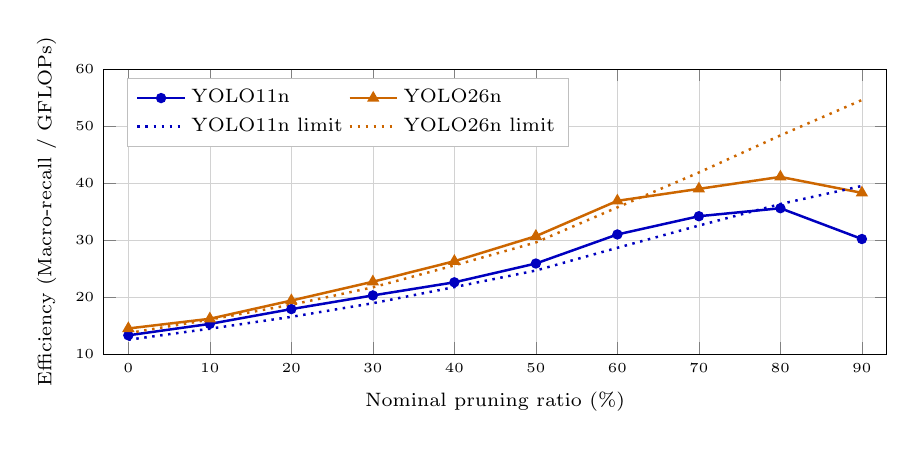
\begin{tikzpicture}
\begin{axis}[
  width=0.95\columnwidth,
  height=5.2cm,
  grid=both,
  grid style={line width=.2pt, draw=gray!25},
  major grid style={line width=.2pt, draw=gray!35},
  tick label style={font=\tiny},
  label style={font=\scriptsize},
  xlabel={Nominal pruning ratio (\%)},
  ylabel={Efficiency (Macro-recall / GFLOPs)},
  xmin=-3, xmax=93,
  xtick={0,10,20,30,40,50,60,70,80,90},
  xminorticks=false,
  ymin=10, ymax=60,
  ytick={10,20,30,40,50,60},
  legend pos=north west,
  legend columns=2,
  legend cell align=left,
  legend style={
    font=\scriptsize,
    draw=gray!50,
    fill=white,
    inner xsep=3pt,
    inner ysep=2pt
  }
]

% YOLO11N efficiency
\addplot[color=blue!75!black, mark=*, mark size=1.4pt, line width=0.9pt] coordinates {
  (0,  13.3)
  (10, 15.3)
  (20, 17.9)
  (30, 20.3)
  (40, 22.6)
  (50, 25.9)
  (60, 31.0)
  (70, 34.2)
  (80, 35.6)
  (90, 30.2)
};
\addlegendentry{YOLO11n}

% YOLO26N efficiency
\addplot[color=orange!80!black, mark=triangle*, mark size=1.7pt, line width=0.9pt] coordinates {
  (0,  14.5)
  (10, 16.2)
  (20, 19.4)
  (30, 22.7)
  (40, 26.3)
  (50, 30.7)
  (60, 36.9)
  (70, 39.0)
  (80, 41.1)
  (90, 38.3)
};
\addlegendentry{YOLO26n}

% YOLO11N borderline: (86.4 - 5) / GFLOPs = 81.4 / GFLOPs
\addplot[color=blue!75!black, dotted, line width=0.9pt, mark=none] coordinates {
  (0,  12.52)
  (10, 14.46)
  (20, 16.54)
  (30, 18.93)
  (40, 21.76)
  (50, 24.67)
  (60, 28.66)
  (70, 32.56)
  (80, 36.34)
  (90, 39.51)
};
\addlegendentry{YOLO11n limit}

% YOLO26N borderline: (85.8 - 5) / GFLOPs = 80.8 / GFLOPs
\addplot[color=orange!80!black, dotted, line width=0.9pt, mark=none] coordinates {
  (0,  13.69)
  (10, 16.06)
  (20, 18.66)
  (30, 21.72)
  (40, 25.57)
  (50, 29.60)
  (60, 35.75)
  (70, 41.87)
  (80, 48.38)
  (90, 54.59)
};
\addlegendentry{YOLO26n limit}

\end{axis}
\end{tikzpicture}
\caption{Efficiency versus nominal pruning ratio. Dotted lines show the minimum efficiency at which a pruned model still passes the safety check. A solid line below its dotted line of the same color means the model fails.}
\label{fig:pruning_efficiency}
\end{figure}

% ======================================================================
% Tab. Quantization 
% ======================================================================

\begin{table*}[!t]
\renewcommand{\arraystretch}{0.85}
\caption{Unquantized baseline versus INT8 PTQ and QAT at 0--90\% sparsity. The baseline row is the unquantized model. Arrows indicate the better direction; bold marks the best value among safe configurations for each method. The baseline is averaged over three seeds; PTQ and QAT results come from a single seed.}
\label{tab:quantization}
\centering
\footnotesize
\setlength{\tabcolsep}{4pt}
\begin{tabular}{l ccc cccc cccc}
\toprule
 & \multicolumn{3}{c}{\textit{Complexity}} & \multicolumn{4}{c}{\textit{INT8 PTQ}} & \multicolumn{4}{c}{\textit{INT8 QAT}} \\
\cmidrule(lr){2-4}\cmidrule(lr){5-8}\cmidrule(lr){9-12}
Sparsity (\%) & \shortstack{Param.\ red.\\(\%) $\uparrow$} & GFLOPs $\downarrow$ & \shortstack{Size\\(MB) $\downarrow$}
 & Prec.\ $\uparrow$ & Rec.\ $\uparrow$ & $\text{Eff}_{\text{MB}}$ $\uparrow$ & Safe
 & Prec.\ $\uparrow$ & Rec.\ $\uparrow$ & $\text{Eff}_{\text{MB}}$ $\uparrow$ & Safe \\


\midrule
0  & 0.0  & 6.50 & 2.92 & 0.819 & 0.859 & 29.4 & \checkmark & 0.829 & 0.807 & 27.6 & $\times$ \\
10 & 13.5 & 5.63 & 2.60 & 0.797 & 0.877 & 33.7 & \checkmark & 0.917 & 0.845 & 32.5 & \checkmark \\
20 & 24.9 & 4.92 & 2.32 & \textbf{0.920} & 0.862 & 37.2 & \checkmark & 0.869 & 0.838 & 36.1 & \checkmark \\
30 & 35.6 & 4.30 & 2.06 & 0.902 & 0.872 & 42.3 & \checkmark & \textbf{0.932} & 0.894 & 43.4 & \checkmark \\
40 & 44.8 & 3.74 & 1.83 & 0.800 & 0.853 & 46.6 & \checkmark & 0.846 & \textbf{0.896} & 49.0 & \checkmark \\
50 & 52.5 & 3.30 & 1.64 & 0.805 & \textbf{0.907} & 55.3 & \checkmark & 0.893 & 0.881 & 53.7 & \checkmark \\
60 & 59.8 & 2.84 & 1.45 & 0.861 & 0.865 & 59.7 & \checkmark & 0.876 & 0.894 & \textbf{61.7} & \checkmark \\
70 & 65.6 & 2.50 & 1.31 & 0.775 & 0.884 & \textbf{67.5} & \checkmark & 0.948 & 0.546 & 41.7 & $\times$ \\
80 & 70.4 & 2.24 & 1.19 & 0.894 & 0.307 & 25.8 & $\times$ & 0.883 & 0.815 & 68.5 & $\times$ \\
90 & 73.9 & 2.06 & 1.10 & 0.700 & 0.667 & 60.6 & $\times$ & 0.791 & 0.635 & 57.7 & $\times$ \\
\midrule
Unquant. & 0.0 & 6.50 & 5.23
 & \multicolumn{8}{c}{Prec.\ $0.936 \pm 0.012$ \quad Rec.\ $0.864 \pm 0.013$ \quad $\text{Eff}_{\text{MB}}$ 16.5 \quad Safe: \checkmark} \\
\bottomrule
\end{tabular}
\end{table*}

% ======================================================================
% Fig. Quantization Plot
% ======================================================================
\begin{figure}[!t]
\centering
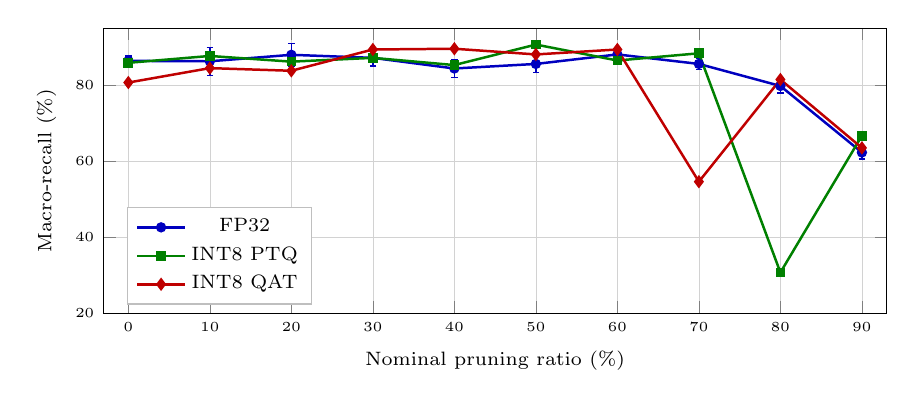
\begin{tikzpicture}
\begin{axis}[
  width=0.95\columnwidth,
  height=5.2cm,
  grid=both,
  grid style={line width=.2pt, draw=gray!25},
  major grid style={line width=.2pt, draw=gray!35},
  tick label style={font=\tiny},
  label style={font=\scriptsize},
  xlabel={Nominal pruning ratio (\%)},
  ylabel={Macro-recall (\%)},
  xmin=-3, xmax=93,
  xtick={0,10,20,30,40,50,60,70,80,90},
  xminorticks=false,
  ymin=20, ymax=95,
  ytick={20,40,60,80},
  legend pos=south west,
  legend style={
    font=\scriptsize,
    draw=gray!50,
    fill=white,
    inner xsep=3pt,
    inner ysep=2pt
  },
  error bars/error bar style={line width=0.5pt, solid},
  error bars/error mark options={line width=0.5pt, mark size=1.2pt, rotate=90}
]

% YOLO11N FP32 (mean +- SD over 3 seeds)
\addplot[color=blue!75!black, mark=*, mark size=1.4pt, line width=0.9pt,
         error bars/.cd, y dir=both, y explicit] coordinates {
  (0,  86.4) +- (0, 1.3)
  (10, 86.3) +- (0, 3.7)
  (20, 88.0) +- (0, 2.9)
  (30, 87.2) +- (0, 2.1)
  (40, 84.4) +- (0, 2.3)
  (50, 85.6) +- (0, 2.3)
  (60, 88.1) +- (0, 1.2)
  (70, 85.6) +- (0, 1.4)
  (80, 79.8) +- (0, 1.8)
  (90, 62.3) +- (0, 1.7)
};
\addlegendentry{FP32}

% YOLO11N INT8 PTQ
\addplot[color=green!50!black, mark=square*, mark size=1.3pt, line width=0.9pt] coordinates {
  (0,  85.9)
  (10, 87.7)
  (20, 86.2)
  (30, 87.2)
  (40, 85.3)
  (50, 90.7)
  (60, 86.5)
  (70, 88.4)
  (80, 30.7)
  (90, 66.7)
};
\addlegendentry{INT8 PTQ}

% YOLO11N INT8 QAT
\addplot[color=red!75!black, mark=diamond*, mark size=1.7pt, line width=0.9pt] coordinates {
  (0,  80.7)
  (10, 84.5)
  (20, 83.8)
  (30, 89.4)
  (40, 89.6)
  (50, 88.1)
  (60, 89.4)
  (70, 54.6)
  (80, 81.5)
  (90, 63.5)
};
\addlegendentry{INT8 QAT}

\end{axis}
\end{tikzpicture}
\caption{YOLO11n macro-recall versus nominal pruning ratio for FP32 (three seeds), INT8 PTQ (single seed), and INT8 QAT (single seed).}
\label{fig:quant_macro_recall}
\end{figure}

Phase~I compares two ways of shrinking the detector: structured $\ell_1$-norm channel pruning (Fig.~\ref{fig:pruning_efficiency}) and INT8 quantization (Fig.~\ref{fig:quant_macro_recall}). Pruning is applied to YOLO11n and YOLO26n at nominal ratios from 10\% to 90\% in 10-point steps. Quantization is applied to pruned YOLO11n models at every ratio and evaluated against the unquantized baseline. All models use the fixed threshold $\tau = 0.5$ on the held-out test split. Complete results are in Tables~\ref{tab:pruning_fixed_tau} and~\ref{tab:quantization}. Five findings stand out:
\begin{itemize}
\item \emph{Pruning headroom.} YOLO11n macro-recall stays within 1.0~pp of its 86.4\% baseline at every ratio up to 70\% pruning, then drops to 79.8\% at 80\% and collapses to 62.3\% at 90\%. YOLO26n is less resilient: recall stays within 2.4~pp of its 85.8\% baseline up to 60\% pruning, then falls to 75.2\% at 70\%.
\item \emph{Class sensitivity.} Yawning, already the weakest class at baseline, sets the worst-class recall at every ratio from 70\% up, with YOLO11n yawning recall collapsing to 16.2\% at 90\% pruning. Phone use, the majority class (81\% of positives), shows the smallest variation across ratios.
\item \emph{Precision stability.} Precision remains between 91.7\% and 95.9\% at every ratio for both architectures; structured pruning degrades recall, not precision.
\item \emph{Cost savings.} At 70\% pruning, YOLO11n has 890K parameters (vs.\ 2.59M baseline), 2.50~GFLOPs (vs.\ 6.50), and a 2.01~MB checkpoint (vs.\ 5.23~MB)---a 65.6\% parameter reduction. Savings fall short of the nominal ratio at high sparsity because detection heads and spatial attention modules are excluded from pruning; at 90\%, total parameters fall by only 73.9\%.
\item \emph{Quantization.} In single-seed runs, INT8 PTQ keeps macro-recall at 88.4\% at 70\% pruning (matching the FP32 85.6\%) while compressing the checkpoint to 1.31~MB. QAT at 60\% pruning recovers 89.4\% macro-recall (vs.\ 88.1\% FP32) in 1.45~MB. Both INT8 formats lower precision relative to their FP32 counterparts. 
\end{itemize}

\subsection{Phase 2: Input-Side Optimization}
\newcommand{\seearrow}{\rotatebox[origin=c]{-20}{$\rightarrow$}}

% ======================================================================
% Tab. Main Input Table
% ======================================================================

\begin{table*}[!t]
\renewcommand{\arraystretch}{0.9}
\caption{Detection performance and computational cost across input resolutions and framing methods over 3 seeds. Precision, recall, and F1 are computed at the optimized threshold $\tau^*$. $^*$400$\times$400 crop upscaled to 640$\times$640. Arrows indicate the better direction; bold marks the best value among safe configurations.}
\label{tab:accuracy}
\centering
\footnotesize
\setlength{\tabcolsep}{4pt}
\begin{tabular}{l ccc cc cc c}
\toprule
 & \multicolumn{3}{c}{\textit{Detection at $\tau^*$}} & \multicolumn{2}{c}{\textit{mAP}} & \multicolumn{2}{c}{\textit{Cost \& efficiency}} & \\
\cmidrule(lr){2-4}\cmidrule(lr){5-6}\cmidrule(lr){7-8}
Input (px) & Precision $\uparrow$ & Recall $\uparrow$ & F1 $\uparrow$ & @0.5 $\uparrow$ & @0.5:0.95 $\uparrow$ & GFLOPs $\downarrow$ & Recall/GFLOPs $\uparrow$ & Safe \\
\midrule
\multicolumn{9}{l}{\textit{Baseline}} \\
640 & $0.882\pm0.020$ & $0.846\pm0.016$ & $0.863\pm0.002$ & $\mathbf{0.889}\pm\mathbf{0.019}$ & $0.548\pm0.003$ & 6.4 & 0.132 & \checkmark \\
320 & $\mathbf{0.913}\pm\mathbf{0.019}$ & $0.813\pm0.030$ & $0.859\pm0.009$ & $0.886\pm0.008$ & $0.560\pm0.004$ & 1.6 & 0.508 & \checkmark \\
160 & $0.875\pm0.009$ & $0.814\pm0.011$ & $0.844\pm0.003$ & $0.837\pm0.002$ & $0.504\pm0.000$ & 0.4 & 2.035 & \checkmark \\
80  & $0.889\pm0.018$ & $0.704\pm0.022$ & $0.786\pm0.016$ & $0.772\pm0.027$ & $0.437\pm0.016$ & 0.1 & 7.040 & $\times$ \\
\midrule
\multicolumn{9}{l}{\textit{Cropped}} \\
640$^*$ & $0.879\pm0.024$ & $0.816\pm0.028$ & $0.846\pm0.020$ & $0.850\pm0.001$ & $0.571\pm0.010$ & 6.4 & 0.128 & \checkmark \\
320 & $0.865\pm0.030$ & $\mathbf{0.864}\pm\mathbf{0.014}$ & $\mathbf{0.864}\pm\mathbf{0.009}$ & $0.885\pm0.004$ & $\mathbf{0.608}\pm\mathbf{0.016}$ & 1.6 & 0.540 & \checkmark \\
160 & $0.886\pm0.014$ & $0.817\pm0.022$ & $0.850\pm0.013$ & $0.845\pm0.010$ & $0.566\pm0.017$ & 0.4 & \textbf{2.043} & \checkmark \\
80  & $0.871\pm0.041$ & $0.730\pm0.058$ & $0.791\pm0.019$ & $0.813\pm0.011$ & $0.514\pm0.008$ & 0.1 & 7.300 & $\times$ \\
\midrule
\multicolumn{9}{l}{\textit{Collage}} \\
640 & $0.853\pm0.012$ & $0.811\pm0.013$ & $0.832\pm0.012$ & $0.805\pm0.016$ & $0.526\pm0.012$ & 6.4 & 0.127 & \checkmark \\
320 & $0.868\pm0.011$ & $0.826\pm0.015$ & $0.847\pm0.006$ & $0.819\pm0.006$ & $0.538\pm0.006$ & 1.6 & 0.516 & \checkmark \\
160 & $0.838\pm0.008$ & $0.698\pm0.030$ & $0.761\pm0.020$ & $0.716\pm0.012$ & $0.452\pm0.011$ & 0.4 & 1.745 & $\times$ \\
80  & $0.701\pm0.079$ & $0.584\pm0.012$ & $0.635\pm0.035$ & $0.520\pm0.047$ & $0.294\pm0.015$ & 0.1 & 5.840 & $\times$ \\
\bottomrule
\end{tabular}
\end{table*}

% ======================================================================
% Fig. pareto3d 
% ======================================================================
\begin{figure}[!t]
\centering
\pgfplotsset{
  mBase/.style={color=blue!75!black},
  mCrop/.style={color=teal!70!black},
  mColl/.style={color=orange!80!black},
  s640/.style={mark=*,        mark size=2.6pt},
  s320/.style={mark=triangle*,mark size=3.2pt},
  s160/.style={mark=square*,  mark size=2.6pt},
  s80/.style={mark=diamond*,  mark size=3.4pt},
  pt/.style={only marks, forget plot},
}
\begin{tikzpicture}
\begin{axis}[
    width=\columnwidth,
    height=0.9\columnwidth,
    view={125}{22},
    xlabel={F1 $\swarrow$},
    ylabel={Efficiency (Recall/GFLOPs) $\seearrow$},
    zlabel={mAP@0.5 $\rightarrow$},
    xmin=0.62, xmax=0.88,
    xtick={0.65,0.75,0.85},
    ymode=log, log basis y=10,
    ymin=0.1, ymax=10,
    ytick={0.1,1,10},
    yticklabels={$10^{-1}$,$10^{0}$,$10^{1}$},
    zmin=0.50, zmax=0.91,
    ztick={0.5,0.6,0.7,0.8,0.9},
    grid=major,
    grid style={dashed,gray!30},
    tick label style={font=\tiny},
    label style={font=\scriptsize},
    legend to name=pareto3dlegend,
    legend columns=5,
    legend cell align=left,
    legend style={
        font=\scriptsize,
        draw=none,
        /tikz/column sep=4pt,
        /tikz/row sep=1pt,
    },
]
% ---------- Vertical drop lines (solid gray to zmin = 0.50) ----------
\draw[gray, solid] (axis cs:0.863,0.132,0.50) -- (axis cs:0.863,0.132,0.889);
\draw[gray, solid] (axis cs:0.846,0.128,0.50) -- (axis cs:0.846,0.128,0.850);
\draw[gray, solid] (axis cs:0.832,0.127,0.50) -- (axis cs:0.832,0.127,0.805);

\draw[gray, solid] (axis cs:0.859,0.508,0.50) -- (axis cs:0.859,0.508,0.886);
\draw[gray, solid] (axis cs:0.864,0.540,0.50) -- (axis cs:0.864,0.540,0.885);
\draw[gray, solid] (axis cs:0.847,0.516,0.50) -- (axis cs:0.847,0.516,0.819);

\draw[gray, solid] (axis cs:0.844,2.035,0.50) -- (axis cs:0.844,2.035,0.837);
\draw[gray, solid] (axis cs:0.850,2.043,0.50) -- (axis cs:0.850,2.043,0.845);
\draw[gray, solid] (axis cs:0.761,1.745,0.50) -- (axis cs:0.761,1.745,0.716);

\draw[gray, solid] (axis cs:0.786,7.040,0.50) -- (axis cs:0.786,7.040,0.772);
\draw[gray, solid] (axis cs:0.791,7.300,0.50) -- (axis cs:0.791,7.300,0.813);
\draw[gray, solid] (axis cs:0.635,5.840,0.50) -- (axis cs:0.635,5.840,0.520);

% ---------- 640 x 640 (circle) ----------
\addplot3[pt,s640,mBase] coordinates {(0.863,0.132,0.889)};
\addplot3[pt,s640,mCrop,mark options={fill=white}] coordinates {(0.846,0.128,0.850)};
\addplot3[pt,s640,mColl] coordinates {(0.832,0.127,0.805)};

% ---------- 320 x 320 (triangle) ----------
\addplot3[pt,s320,mBase] coordinates {(0.859,0.508,0.886)};
\addplot3[pt,s320,mCrop] coordinates {(0.864,0.540,0.885)};
\addplot3[pt,s320,mColl] coordinates {(0.847,0.516,0.819)};

% ---------- 160 x 160 (square) ----------
\addplot3[pt,s160,mBase] coordinates {(0.844,2.035,0.837)};
\addplot3[pt,s160,mCrop] coordinates {(0.850,2.043,0.845)};
\addplot3[pt,s160,mColl] coordinates {(0.761,1.745,0.716)};

% ---------- 80 x 80 (diamond) ----------
\addplot3[pt,s80,mBase] coordinates {(0.786,7.040,0.772)};
\addplot3[pt,s80,mCrop] coordinates {(0.791,7.300,0.813)};
\addplot3[pt,s80,mColl] coordinates {(0.635,5.840,0.520)};

% ---------- highlight: 320 x 320 Cropped (open ring) ----------
\addplot3[pt,mark=o,mark size=7pt,line width=1pt,mCrop]
    coordinates {(0.864,0.540,0.885)};

% -- row 1: Method (colour; neutral circle shape) --
\addlegendimage{empty legend}                      \addlegendentry{\textbf{Method}}
\addlegendimage{only marks,mark=*,mark size=2.6pt,mBase} \addlegendentry{Baseline}
\addlegendimage{only marks,mark=*,mark size=2.6pt,mCrop} \addlegendentry{Cropped}
\addlegendimage{only marks,mark=*,mark size=2.6pt,mColl} \addlegendentry{Collage}
\addlegendimage{empty legend}                      \addlegendentry{}

% -- row 2: Input resolution (shape; neutral grey colour) --
\addlegendimage{empty legend}                      \addlegendentry{\textbf{Input (px)}}
\addlegendimage{only marks,s640,color=black!70}    \addlegendentry{640}
\addlegendimage{only marks,s320,color=black!70}    \addlegendentry{320}
\addlegendimage{only marks,s160,color=black!70}    \addlegendentry{160}
\addlegendimage{only marks,s80, color=black!70}    \addlegendentry{80}
\end{axis}
\end{tikzpicture}
\vspace{3pt}
\pgfplotslegendfromname{pareto3dlegend}
\caption{Three-dimensional comparison of input configurations using F1, efficiency (Recall/GFLOPs), and mAP@0.5. Marker color encodes the spatial framing method (Baseline, Cropped, Collage) and marker shape encodes the network input resolution (640, 320, 160, 80\,px). The ringed 320$\times$320 Cropped configuration is the best overall compromise. The hollow circle marks Cropped at 640\,px, a 400$\times$400 crop upscaled to 640$\times$640.}
\label{fig:pareto3d}
\end{figure}

Phase~2 compares three input strategies (Fig.~\ref{fig:preprocessing_comparison}): the full frame (Baseline), a cropped region of interest (Cropped), and an overlapping collage (Collage). Evaluated across 3 seeds, each is evaluated at network input sizes of 640, 320, 160, and 80 pixels. Precision, recall, and F1 use the frozen threshold $\tau^*$ (Section~\ref{sec:threshold}), and the complete detection and timing results are listed in Table~\ref{tab:accuracy} and Fig.~\ref{fig:pareto3d}. Five findings stand out:
\begin{itemize}
\item \emph{Resolution headroom.} F1 accuracy holds down to 320 pixels ($0.859$ vs.\ $0.863$ at 640), and the loss below that is concentrated in yawning.
%\item \emph{Latency saturation.} Below 320 pixels, compute reductions yield diminishing speedups: scaling from 320 down to 80 pixels cuts GFLOPs by $16\times$ (1.6 to 0.1~GFLOPs).
\item \emph{RoI cropping.} It gives the best balance of accuracy and speed, but its effect depends on the behavior class: yawning recall benefits from tighter driver framing at 320 pixels (0.879 vs.\ 0.823 baseline), while classes requiring peripheral visibility remain steady.
\item \emph{Collage.} It does not help at any size; it trails the Baseline at every resolution as spatial partitioning fractures contextual continuity across tile seams.
\item \emph{Best configuration.} Cropped at 320 pixels achieves the optimal operating point: recall 0.864, F1 0.864, and mAP@0.5:0.95 0.608 at one quarter of the 640-pixel cost (1.6 vs.\ 6.4~GFLOPs), A second cheap option is cropped at 160 pixels achieves:  recall 0.817, F1 0.850, and mAP@0.5:0.95 0.566 at one-sixteenth of the 640-pixel cost (0.4 vs.\ 6.4~GFLOPs)
\end{itemize}

%%%%%%%%%%%%%%%%%%%%%%%%%%%%%%%%%%%%%%%%%%%%%%%%%%%%%%%%%%%%%%%%%%%%%%%%
% CRITICAL DISCLAIMER — READ BEFORE USING THIS FILE
%
% 1. AI-ASSISTED DRAFT. This LaTeX was generated or edited with AI
%    assistance. Treat it as a strong starting point, not a submission-
%    ready file — read every section, equation, and citation yourself
%    before you submit.
%
% 2. RECOMPILE AND VISUALLY CHECK. These fixes follow IEEE's documented
%    style rules, not a live compile on your machine. Build this file in
%    your own LaTeX environment and visually inspect every equation,
%    table, and figure before you trust the rendering.
%
% 3. CONFIRM YOUR VENUE'S TEMPLATE. This follows IEEE's generic
%    conference template (IEEEtran, conference mode). Your specific
%    conference or journal may require a different template, page limit,
%    or formatting variant — check that venue's author instructions
%    before submitting.
%%%%%%%%%%%%%%%%%%%%%%%%%%%%%%%%%%%%%%%%%%%%%%%%%%%%%%%%%%%%%%%%%%%%%%%%

\subsection{Phase 3: System Co-design}
\begin{table*}[!t]
\renewcommand{\arraystretch}{1.15}
\caption{Co-design study results (mean $\pm$ SD over three seeds) comparing the pruned + quantized pipeline at two cropped input resolutions against the native FP32 baselines at a fixed confidence threshold $\tau = 0.50$. PTQ: post-training quantization.}
\label{tab:codesign_study}
\centering
\scriptsize
\setlength{\tabcolsep}{3.2pt}
\begin{tabular}{l c c c r r r cc}
\toprule
\multicolumn{4}{c}{Model Specification} 
& \multicolumn{3}{c}{Cost / Footprint $\downarrow$} 
& \multicolumn{2}{c}{Accuracy at $\tau = 0.50$ (\%) $\uparrow$} \\
\cmidrule(lr){1-4}
\cmidrule(lr){5-7}
\cmidrule(lr){8-9}
Architecture & Input Res. & Sparsity & Quant. 
& Params & GFLOPs & Size (MB) 
& Precision & Macro-Recall \\
\midrule
\multicolumn{9}{l}{\textit{Co-Design Pipeline (Cropped + Pruned + INT8)}} \\
YOLO11N & 320$\times$320 Crop & Pruned 70\% & PTQ INT8 
& 890{,}533 & 0.614 & 1.19 
& $77.4 \pm 6.0$ & $79.1 \pm 1.2$ \\
YOLO11N & 160$\times$160 Crop & Pruned 70\% & PTQ INT8 
& 890{,}533 & 0.153 & 1.16 
& $74.1 \pm 12.6$ & $72.3 \pm 0.9$ \\
\midrule
\multicolumn{9}{l}{\textit{Native Baselines (640$\times$640 Native, FP32)}} \\
YOLO11N & 640$\times$640 Native & Base (0\%) & FP32 
& 2.59\,M & 6.50 & 5.23 
& $93.6 \pm 1.2$ & $86.4 \pm 1.3$ \\
YOLO26N & 640$\times$640 Native & Base (0\%) & FP32 
& 2.51\,M & 5.90 & 5.15 
& $95.1 \pm 0.6$ & $85.8 \pm 1.7$ \\
\bottomrule
\end{tabular}
\end{table*}


\begin{figure}[!t]
\centering
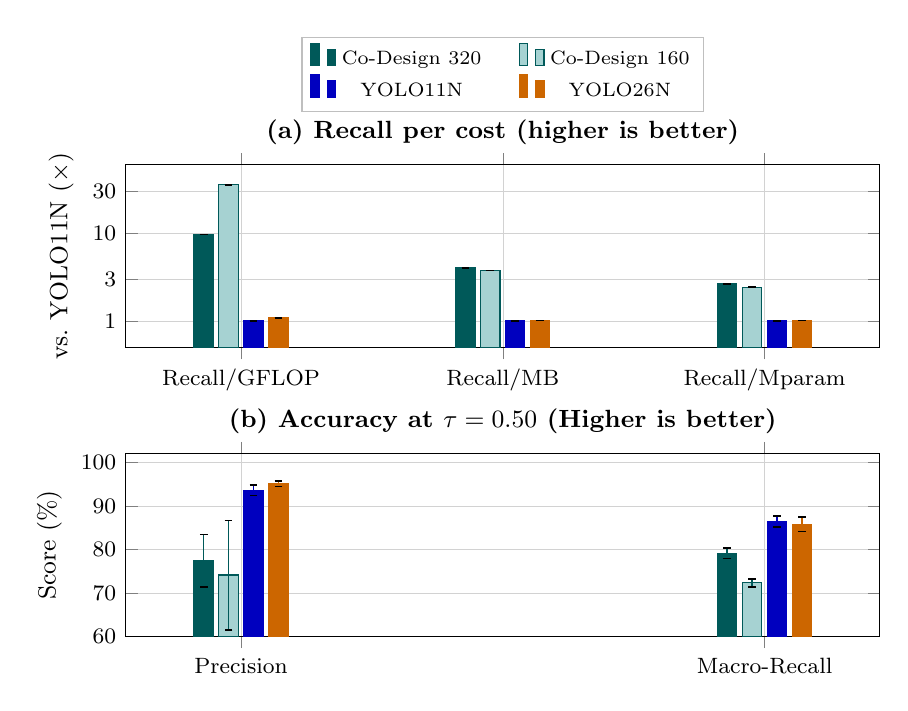
\begin{tikzpicture}
  \begin{groupplot}[
    group style={
      group size=1 by 2,
      vertical sep=1.35cm,
      xlabels at=edge bottom,
      ylabels at=edge left,
    },
    width=0.92\columnwidth,
    height=3.9cm,
    grid=both,
    grid style={line width=.2pt, draw=gray!25},
    major grid style={line width=.2pt, draw=gray!35},
    tick label style={font=\footnotesize},
    label style={font=\small},
    title style={font=\small\bfseries, yshift=-0.5ex},
    legend style={
      font=\scriptsize,
      draw=gray!50,
      fill=white,
      legend columns=2,
      /tikz/every even column/.append style={column sep=0.4cm}
    },
    ybar,
    enlarge x limits=0.22,
    error bars/y dir=both,
    error bars/y explicit,
    error bars/error bar style={line width=0.55pt, solid},
    error bars/error mark options={line width=0.55pt, mark size=1.4pt, rotate=90}
  ]
  % ----------------------------------------------------
  % Panel (a): Recall per unit cost, relative to native
  % YOLO11N (higher = better, log scale)
  % ----------------------------------------------------
  \nextgroupplot[
    title={(a) Recall per cost (higher is better)},
    ylabel={vs.\ YOLO11N ($\times$)},
    ymode=log,
    log origin=infty,
    log ticks with fixed point,
    grid=major,
    ymin=0.5, ymax=60,
    ytick={1, 3, 10, 30},
    symbolic x coords={GFLOP, MB, Param},
    xticklabels={Recall/GFLOP, Recall/MB, Recall/Mparam},
    xtick=data,
    bar width=7pt,
    legend to name=sharedlegend,
  ]
  % Co-Design YOLO11N, 320x320 crop (dark teal)
  \addplot[
    fill=teal!70!black,
    draw=teal!70!black,
  ] coordinates {
    (GFLOP, 9.69) +- (0, 0)
    (MB,    4.02) +- (0, 0)
    (Param, 2.66) +- (0, 0)
  };
  \addlegendentry{Co-Design 320}
  % Co-Design YOLO11N, 160x160 crop (light teal, same outline)
  \addplot[
    fill=teal!35!white,
    draw=teal!70!black,
  ] coordinates {
    (GFLOP, 35.55) +- (0, 0)
    (MB,    3.77)  +- (0, 0)
    (Param, 2.43)  +- (0, 0)
  };
  \addlegendentry{Co-Design 160}
  % Native YOLO11N (blue) -- reference, = 1 by definition
  \addplot[
    fill=blue!75!black,
    draw=blue!75!black,
  ] coordinates {
    (GFLOP, 1.00) +- (0, 0)
    (MB,    1.00) +- (0, 0)
    (Param, 1.00) +- (0, 0)
  };
  \addlegendentry{YOLO11N}
  % Native YOLO26N (orange)
  \addplot[
    fill=orange!80!black,
    draw=orange!80!black,
  ] coordinates {
    (GFLOP, 1.09) +- (0, 0)
    (MB,    1.01) +- (0, 0)
    (Param, 1.02) +- (0, 0)
  };
  \addlegendentry{YOLO26N}
  % ----------------------------------------------------
  % Panel (b): Accuracy (higher = better)
  % ----------------------------------------------------
  \nextgroupplot[
    title={(b) Accuracy at $\tau=0.50$ (Higher is better)},
    ylabel={Score (\%)},
    ymin=60, ymax=102,
    ytick={60, 70, 80, 90, 100},
    symbolic x coords={Precision, Macro-Recall},
    xtick=data,
    bar width=7pt,
  ]
  % Co-Design YOLO11N, 320x320 crop
  \addplot[
    fill=teal!70!black,
    draw=teal!70!black,
  ] coordinates {
    (Precision, 77.4) +- (0, 6.0)
    (Macro-Recall, 79.1) +- (0, 1.2)
  };
  % Co-Design YOLO11N, 160x160 crop
  \addplot[
    fill=teal!35!white,
    draw=teal!70!black,
  ] coordinates {
    (Precision, 74.1) +- (0, 12.6)
    (Macro-Recall, 72.3) +- (0, 0.9)
  };
  % Native YOLO11N
  \addplot[
    fill=blue!75!black,
    draw=blue!75!black,
  ] coordinates {
    (Precision, 93.6) +- (0, 1.2)
    (Macro-Recall, 86.4) +- (0, 1.3)
  };
  % Native YOLO26N
  \addplot[
    fill=orange!80!black,
    draw=orange!80!black,
  ] coordinates {
    (Precision, 95.1) +- (0, 0.6)
    (Macro-Recall, 85.8) +- (0, 1.7)
  };
  \end{groupplot}
  \node[anchor=south] at ($(group c1r1.north)+(0, 0.55cm)$)
    {\pgfplotslegendfromname{sharedlegend}};
\end{tikzpicture}
\caption{Efficiency--accuracy comparison. (a)~Mean macro-recall divided by GFLOPs, model size (MB), or parameters (M), normalized to native YOLO11N (log scale; higher is better) (b)~Precision and macro-recall at $\tau=0.50$ (mean $\pm$ SD over three seeds).}
\label{fig:efficiency_accuracy}
\end{figure}
Phase~3 investigates the compounding benefits of hardware--software co-design by uniting spatial input reduction, structured channel pruning, and post-training quantization (Table~\ref{tab:codesign_study} and Fig.~\ref{fig:efficiency_accuracy}). We evaluate the co-designed YOLO11n pipeline (Cropped input at $320\times 320$ and $160 \times 160$, Pruned 70\%, PTQ INT8) against native full-frame ($640\times 640$, FP32) baselines of YOLO11n and YOLO26n. All results use a fixed operational threshold $\tau = 0.50$ with greedy bipartite matching at $\text{IoU} = 0.50$ on the held-out, subject-disjoint test split (3{,}213 images from three subjects). Each co-design run was trained for up to 80 epochs with early stopping (patience of 15) and a batch size of 16, using three seeds. Four findings stand out:

\begin{itemize}
    \item \emph{Extreme compute scaling.} Compounding RoI cropping with 70\% structural channel pruning cuts computational complexity by over an order of magnitude relative to native YOLO11n ($6.50$\,GFLOPs; $5.90$\,GFLOPs for YOLO26n): GFLOPs drop by $\approx$\textbf{10.6$\times$} to $0.614$ at $320\times 320$ and by $\approx$\textbf{42.5$\times$} to $0.153$ at $160\times 160$. Parameter count falls by $\approx$\textbf{2.9$\times$} ($890{,}533$ vs.\ $2.59$\,M) at both resolutions, since both use the same pruned network.
    
    \item \emph{Embedded footprint compression.} 8-bit post-training quantization on top of pruning shrinks the exported model by $\approx$\textbf{4.4$\times$} ($1.19$\,MB vs.\ $5.23$\,MB for native YOLO11n and $5.15$\,MB for YOLO26n) at $320\times 320$ and by $\approx$\textbf{4.5$\times$} ($1.16$\,MB) at $160\times 160$. This brings the model within reach of microcontroller-class and embedded NPU targets, although the actual fit depends on the memory budget of the target device.

    \item \emph{Recall resilience.} Despite eliminating $>90\%$ of arithmetic operations, the $320\times 320$ pipeline retains a macro-recall of \textbf{79.1\%} ($\pm 1.2\%$), conceding $7.3$ percentage points relative to full-frame YOLO11n ($86.4 \pm 1.3\%$) and $6.7$ points relative to YOLO26n ($85.8 \pm 1.7\%$). The $160\times 160$ variant falls further to $72.3 \pm 0.9\%$, i.e., $14.1$ and $13.5$ points below the two baselines. Macro-recall is stable across seeds at both resolutions.

    \item \emph{Precision trade-off.} Precision drops from $93.6 \pm 1.2\%$ (YOLO11n) and $95.1 \pm 0.6\%$ (YOLO26n) to \textbf{77.4\%} ($\pm 6.0\%$) at $320\times 320$ and to $74.1 \pm 12.6\%$ at $160\times 160$, where per-seed precision ranges from $60.4\%$ to $85.0\%$. This corresponds to a clear rise in false alarms at a fixed $\tau = 0.50$ and is the primary performance concession for the $\approx$10.6$\times$ to $\approx$42.5$\times$ reduction in compute. Because $\tau$ is not re-tuned for the pruned and quantized models, part of this gap may reflect a shift in their confidence calibration, which this study does not isolate.

\subsection{Limitations and Future Work}
\label{sec:limitations}
Several limitations qualify the findings above.
\begin{itemize}
    \item \emph{Single-seed quantization.} The INT8 PTQ and QAT results in Phase~I come from a single seed (Table~\ref{tab:quantization}), and the non-monotonic QAT behavior (e.g., 54.6\% macro-recall at 70\% sparsity versus 81.5\% at 80\%) suggests that run-to-run variance is substantial. These results indicate trends rather than statistically established differences.
    \item \emph{No on-device measurements.} Compute is reported as GFLOPs and storage as checkpoint size, and accuracy was evaluated on a desktop GPU. We did not measure latency, power, or memory use on automotive microcontrollers or NPUs, where INT8 operator support and memory hierarchies can change the realized speedups.
\end{itemize}

Future work should address these points in the following order. First, Quantization experiments should be repeated across multiple seeds, and evaluation should be extended to additional subjects, cabin geometries, and lighting conditions with larger minority-class support. Third, these input strategies should be tested on dedicated automotive microcontrollers and NPUs, where image signal processors (ISPs) can perform hardware-accelerated cropping and format conversion with zero CPU overhead, and where latency and power can be measured directly. Finally, dynamic RoI tracking that follows the driver's head pose could relax fixed camera mounting assumptions while further hardening edge detection robustness across diverse cabin geometries.
\end{itemize}

\section{Conclusion}
This paper examined whether model-level compression and input-level preprocessing, studied separately and then combined, can reduce the cost of edge driver monitoring without violating a safety-critical recall requirement. Using subject-disjoint evaluation on the DMD, we benchmarked structured $\ell_1$-norm channel pruning with INT8 quantization on YOLO11n and YOLO26n, compared static central-crop and overlapping-collage inputs across four resolutions, and combined the strongest settings in a single pipeline.

Three conclusions follow. First, YOLO11n tolerates structured pruning up to 70\% sparsity while remaining within the 5-pp safety recall floor, whereas YOLO26n tolerates only 60\%.  Second, a static central crop at $320\times320$ matches the full-frame macro-F1 at one quarter of the compute, while the overlapping collage never improves on the full frame, as tile seams break contextual continuity. Third, the two levers compound: a 70\%-pruned, PTQ INT8 YOLO11n on a $320\times320$ crop reduces compute by $10.6\times$ (0.614~GFLOPs) and storage by $4.4\times$ (1.19~MB), and the $160\times160$ variant reduces compute by $42.5\times$ (0.153~GFLOPs).

These gains are not free. At a fixed threshold of $\tau=0.50$, the $320\times320$ pipeline retains 79.1\% macro-recall (91.6\% of the 86.4\% baseline), a 7.3-pp drop and the $160\times160$ variant drops 14.1~pp. Precision also falls from 93.6\% to 77.4\% and 74.1\%, respectively. The co-designed pipeline is therefore best viewed as an efficiency-oriented operating point that requires recovery of recall before safety-critical deployment, rather than as a drop-in replacement for the native detector. Several limitations qualify these findings: the test split contains only 33 yawning and 28 hand-over-mouth frames, quantization results in Phase~I come from a single seed, and no latency was measured on target embedded hardware. Future work will address these points through on-device evaluation on automotive microcontrollers and NPUs.

% Bibliography
\begin{thebibliography}{00}
\bibitem{b1} J. Guo, W. Ouyang, and D. Xu, ``Multi-dimensional pruning: A unified framework for model compression,'' in \emph{Proc. IEEE/CVF Conf. Comput. Vis. Pattern Recognit. (CVPR)}, 2020, pp. 1508--1517.
\bibitem{b2} A. Vina, ``Pruning and quantization in computer vision: A quick guide,'' Ultralytics Blog, Jul. 11, 2025. Accessed: Sep. 29, 2026. [Online]. Available: \url{https://www.ultralytics.com/blog/pruning-and-quantization-in-computer-vision-a-quick-guide}
\bibitem{b3} Y. He, P. Liu, L. Zhu, and Y. Yang, ``Filter pruning by switching to neighboring CNNs with good attributes,'' \emph{IEEE Trans. Neural Netw. Learn. Syst.}, pp. 1--13, 2022, doi: 10.1109/TNNLS.2022.3149332.
\bibitem{b4} Z. Wang, C. Li, and X. Wang, ``Convolutional neural network pruning with structural redundancy reduction,'' in \emph{Proc. IEEE/CVF Conf. Comput. Vis. Pattern Recognit. (CVPR)}, 2021, pp. 14913--14922.
\bibitem{b5} Z. Li, B. Ni, T. Li, and W. Gao, ``Residual quantization for low bit-width neural networks,'' \emph{IEEE Trans. Multimedia}, vol. 25, pp. 214--227, 2023, doi: 10.1109/TMM.2021.3124095.
\bibitem{b6} S. Li \emph{et al.}, ``Distilling a powerful student model via online knowledge distillation,'' \emph{IEEE Trans. Neural Netw. Learn. Syst.}, pp. 1--10, 2022, doi: 10.1109/TNNLS.2022.3152732.
\bibitem{b8} S. Han, H. Mao, and W. J. Dally, ``Deep compression: Compressing deep neural networks with pruning, trained quantization and Huffman coding,'' in \emph{Proc. Int. Conf. Learn. Represent. (ICLR)}, 2016.
\bibitem{b9} H. Li, A. Kadav, I. Durdanovic, H. Samet, and H. P. Graf, ``Pruning filters for efficient ConvNets,'' in \emph{Proc. Int. Conf. Learn. Represent. (ICLR)}, 2017.
\bibitem{b10} Y. He, X. Zhang, and J. Sun, ``Channel pruning for accelerating very deep neural networks,'' in \emph{Proc. IEEE Int. Conf. Comput. Vis. (ICCV)}, 2017, pp. 1389--1397.
\bibitem{b11} Z. Liu, J. Li, Z. Shen, G. Huang, S. Yan, and C. Zhang, ``Learning efficient convolutional networks through network slimming,'' in \emph{Proc. IEEE Int. Conf. Comput. Vis. (ICCV)}, 2017, pp. 2736--2744.
\bibitem{b12} G. Fang, X. Ma, M. Song, M. B. Mi, and X. Wang, ``DepGraph: Towards any structural pruning,'' in \emph{Proc. IEEE/CVF Conf. Comput. Vis. Pattern Recognit. (CVPR)}, 2023, pp. 16091--16101.
\bibitem{b13} B. Jacob, S. Kligys, B. Chen, M. Zhu, M. Tang, A. Howard, H. Adam, and D. Kalenichenko, ``Quantization and training of neural networks for efficient integer-arithmetic-only inference,'' in \emph{Proc. IEEE/CVF Conf. Comput. Vis. Pattern Recognit. (CVPR)}, 2018, pp. 2704--2713.
\bibitem{b14} R. Krishnamoorthi, ``Quantizing deep convolutional networks for efficient inference: A whitepaper,'' arXiv:1806.08342, 2018.
\bibitem{b15} C.-Y. Wang, A. Bochkovskiy, and H.-Y. M. Liao, ``YOLOv7: Trainable bag-of-freebies sets new state-of-the-art for real-time object detectors,'' in \emph{Proc. IEEE/CVF Conf. Comput. Vis. Pattern Recognit. (CVPR)}, 2023, pp. 7464--7475.
\bibitem{b16} A. Wang, H. Chen, L. Liu, K. Chen, Z. Lin, J. Han, and G. Ding, ``YOLOv10: Real-time end-to-end object detection,'' in \emph{Proc. Adv. Neural Inf. Process. Syst. (NeurIPS)}, vol. 37, 2024.
\bibitem{b17} R. Khanam and M. Hussain, ``YOLOv11: An overview of the key architectural enhancements,'' arXiv:2410.17725, 2024.
\bibitem{b18} F. O. Unel, B. O. Ozkalayci, and C. Cigla, ``The power of tiling for small object detection,'' in \emph{Proc. IEEE/CVF Conf. Comput. Vis. Pattern Recognit. Workshops (CVPRW)}, 2019, pp. 582--591.
\bibitem{b19} M. Najibi, B. Singh, and L. S. Davis, ``AutoFocus: Efficient multi-scale inference,'' in \emph{Proc. IEEE/CVF Int. Conf. Comput. Vis. (ICCV)}, 2019, pp. 9745--9755.
\bibitem{b20} J. D. Ortega, N. Kose, P. Ca\~{n}as, M.-A. Chao, A. Unnervik, M. Nieto, O. Otaegui, and L. Salgado, ``DMD: A large-scale multi-modal driver monitoring dataset for attention and alertness analysis,'' in \emph{Proc. Eur. Conf. Comput. Vis. Workshops (ECCVW)}, 2020, pp. 387--405.
\bibitem{b21} Y. Abouelnaga, H. M. Eraqi, and M. N. Moustafa, ``Real-time distracted driver posture classification,'' arXiv:1706.09498, 2017.
\bibitem{b22} A. Kashevnik, R. Shchedrin, C. Kaiser, and A. Stocker, ``Driver distraction detection methods: A literature review and framework,'' \emph{IEEE Access}, vol. 9, pp. 60063--60076, 2021.
\bibitem{euroncap2026driver}
Euro NCAP, ``Safe Driving: Driver Engagement Protocol,'' Version 1.2, Euro NCAP, Leuven, Belgium, Jul. 2026. [Online]. Available: \url{https://cdn.euroncap.com/cars/assets/Euro_NCAP_Protocol_Safe_Driving_Driver_Engagement_v1_2_ebce03a443.pdf}
\bibitem{isots5283} \textit{Road Vehicles: Driver Readiness and Intervention Management, Part 1: Partial Automation (Level 2)}, ISO/TS 5283-1:2025, International Organization for Standardization, Geneva, Switzerland, Oct. 2025. [Online]. Available: \url{https://www.iso.org/standard/85035.html}

\end{thebibliography}

\end{document}